% DESENVOLVIMENTO--------------------------------------------------------

\chapter{DESENVOLVIMENTO}
\label{chap:desenvolvimento}

\section{DIAGRAMA CASO DE USO}
\label{sec:diagramacasodeuso}

Neste tópico, será apresentado o diagrama de caso de uso, o qual é responsável por mostrar quais as funcionalidades de um sistema, e também quais os usuários com os quais interagem. De forma simples, é semelhante a um mapa que descreve os objetivos dos usuários ao usar o sistema.

\begin{figure}[H]
    \centering
    \caption{Diagrama de Caso de Uso}
    \label{fig:casoDeUso}
    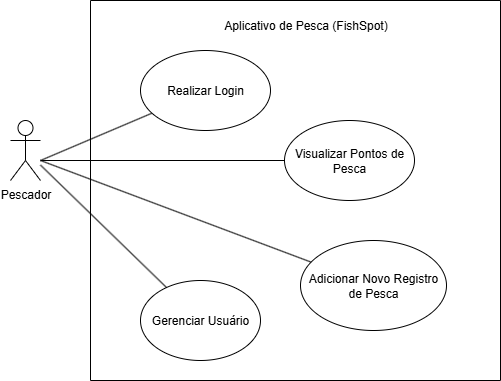
\includegraphics[scale=0.8]{./dados/figuras/diagrama-de-caso-de-uso.png}
    \fonte{\citeonline{DrawIO}}
\end{figure}


\section{DIAGRAMA DE CLASSE}
\label{sec:diagramadeclasse}

O diagrama de classe constitui uma ferramenta muito utilizada para a modelagem estática e estrutural de um sistema. A representação das classes, dos atributos, dos métodos e também suas relações, de forma visual, facilita a compreensão da arquitetura lógica do software.

\begin{figure}[H]
    \centering
    \caption{Diagrama de Classe}
    \label{fig:casoDeUso}
    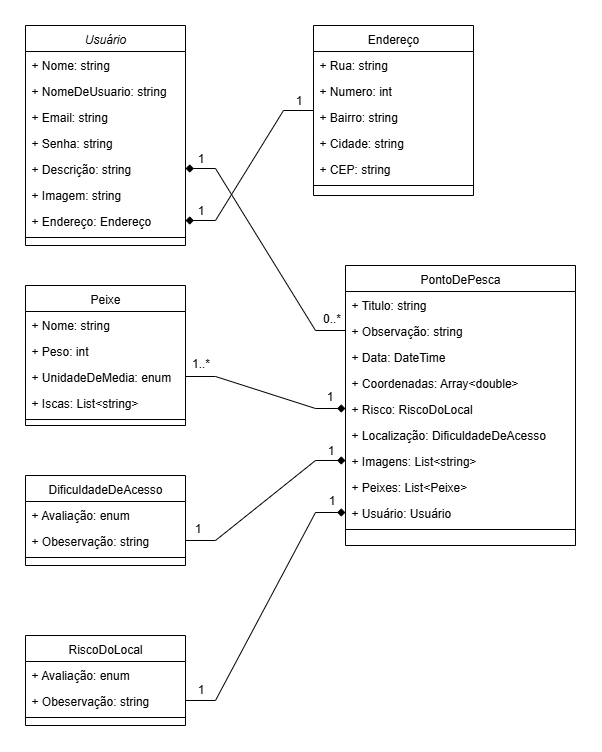
\includegraphics[scale=0.70]{./dados/figuras/diagrama-de-classe.png}
    \fonte{\citeonline{DrawIO}}
\end{figure}

\section{LEVANTAMENTO DE REQUISITOS}\label{sec:levantamentoderequisitos}

De acordo com \citeonline{fernandoCunha2025}, os requisitos funcionais são aqueles que representam funcionalidades às quais estão relacionados a ações dentro da solução proposta. Enquanto os funcionais estão relacionados a ações, os requisitos não funcionais estão relacionados a descrever a forma como serão feitos.

A \autoref{tab:tb-rf-realizar-login} aborda os requisitos para a realização do login, onde o pescador informa as credenciais de acesso, e recebe permissões para navegação dentro da aplicação. Além disso, são descritos seus requisitos não funcionais atrelados.

\begin{table}[h!]
    \centering
    \caption[Requisitos de Autenticação do Usuário]{Requisitos de Autenticação do Usuário
    \label{tab:tb-rf-realizar-login}}
    \setlength{\extrarowheight}{2pt}
    \begin{tabular}{|l!{\vrule width 1pt}p{0.55\textwidth}|c|c|}
        \hline
        \textbf{RF-1} & \multicolumn{3}{|l|}{Realizar Login} \\
        \hline
        \multicolumn{4}{|p{0.9\textwidth}|}{\textbf{Descrição detalhada:} } \\
        \hline
        \multicolumn{4}{|c|}{\textbf{REQUISITOS NÃO FUNCIONAIS ASSOCIADOS}} \\
        \hline
        \textbf{Nome} & \textbf{Restrição} & \textbf{Categoria} & \textbf{Desejável} \\
        \hline
        RNF1.1 & Os dados sensíveis do usuário devem ser criptografados durante o processo de autenticação & Segurança & Obrigatório \\
        \hline
        RNF1.2 & A duração do processo de autenticação não deve ser longo  & Desempenho & Obrigatório \\
        \hline
        RNF1.3 & O usuário não deve conseguir acessar o aplicativo sem ser autenticado & Usabilidade & Obrigatório \\
        \hline
        RNF1.4 & A interface deve seguir os padrões gerais de design para deixar mais intuitiva e acessível & Usabilidade & Obrigatório \\
        \hline
    \end{tabular}
    \fonte{Fonte: Produzido pelo Autor}
\end{table}

A \autoref{tab:tb-rf-visualizar-pontos-pesca} descreve os requisitos para visualizar um ponto de pesca, onde o usuário visualiza todos os pontos de pesca cadastrados, bem como seus detalhes. São detalhados também os requisitos não funcionais relacionados, dentre eles visualização do mapa, cálculos de geolocalização, localização atual do usuário e etc.

\begin{table}[h!]
    \centering
    \caption[Requisitos para Visualização Pontos de Pesca]{Requisitos para Visualização de Pontos de Pesca
    \label{tab:tb-rf-visualizar-pontos-pesca}}
    \setlength{\extrarowheight}{2pt}
    \begin{tabular}{|l!{\vrule width 1pt}p{0.55\textwidth}|c|c|}
        \hline
        \textbf{RF-2} & \multicolumn{3}{|l|}{Visualizar Pontos de Pesca} \\
        \hline
        \multicolumn{4}{|p{0.9\textwidth}|}{\textbf{Descrição detalhada:} } \\
        \hline
        \multicolumn{4}{|c|}{\textbf{REQUISITOS NÃO FUNCIONAIS ASSOCIADOS}} \\
        \hline
        \textbf{Nome} & \textbf{Restrição} & \textbf{Categoria} & \textbf{Desejável} \\
        \hline
        RNF2.1 & Durante visualização dos pontos de pesca, dados sensíveis dos outros usuários não devem ser expostos & Segurança & Obrigatório \\
        \hline
        RNF2.2 & Os pontos de pesca devem ser exibidos em um mapa, semelhante às aplicações Waze, Google Maps e etc. & Usabilidade & Obrigatório \\
        \hline
        RNF2.3 & Deve ser possivel visualizar os pontos de pesca de forma singular, exibindo detalhes do registro feito & Usabilidade & Obrigatório \\
        \hline
        RNF2.4 & Deve ser possivel visualizar as fotos registradas nos detalhes do ponto de pesca  & Usabilidade & Desejável \\
        \hline
        RNF2.5 & As informações devem ser exibidas de forma fluidas e o mapa não deve demorar para renderizar os pontos de pesca & Desempenho & Obrigatório \\
        \hline
    \end{tabular}
    \fonte{Fonte: Produzido pelo Autor}
\end{table}

Os requisitos relacionados ao cadastro de um novo ponto de pesca é representado pela \autoref{tab:tb-rf-novo-registro-pesca}, onde detalha as principais características da funcionalidade, também como seus requisitos não funcionais.

\begin{table}[h!]
    \centering
    \caption[Requisitos de Cadastro de Pontos de Pesca]{Requisitos de Cadastro de Pontos de Pesca
    \label{tab:tb-rf-novo-registro-pesca}}
    \setlength{\extrarowheight}{2pt}
    \begin{tabular}{|l!{\vrule width 1pt}p{0.55\textwidth}|c|c|}
        \hline
        \textbf{RF-3} & \multicolumn{3}{|l|}{Adicionar Novo Registro de Pesca} \\
        \hline
        \multicolumn{4}{|p{0.9\textwidth}|}{\textbf{Descrição detalhada:} } \\
        \hline
        \multicolumn{4}{|c|}{\textbf{REQUISITOS NÃO FUNCIONAIS ASSOCIADOS}} \\
        \hline
        \textbf{Nome} & \textbf{Restrição} & \textbf{Categoria} & \textbf{Desejável} \\
        \hline
        RNF3.1 & Deve ser possível incluir fotos dos peixes capturados durante a pesca & Usabilidade & Obrigatório  \\
        \hline
        RNF3.2 & As iscas utilizadas durante o processo devem ser incluídas & Usabilidade & Obrigatório \\
        \hline
        RNF3.3 & Informações sobre o percurso e sobre riscos devem ser informadas & Usabilidade & Desejavel \\
        \hline
        RNF3.4 & A aplicação deve ser rápida para persistir os dados informados & Desempenho & Obrigatório \\
        \hline
        RNF3.5 & Os dados devem ser armazenados corretamente, para que a confiabilidade das informações sejam mantidas & Segurança & Obrigatório  \\
        \hline
    \end{tabular}
    \fonte{Fonte: Produzido pelo Autor}
\end{table}

Na \autoref{tab:tb-rf-gerenciar-usuario}, os requisitos para gerenciar o usuário são descritos. Nesta funcionalidade é feito o gerenciamento dos dados do usuário, o gerenciamento esta atrelado a incluir, editar e também visualizar os dados dos pescadores.

\begin{table}[h!]
    \centering
    \caption[Requisitos de Gerenciamento do Usuário]{Requisitos de Gerenciamento do Usuário
    \label{tab:tb-rf-gerenciar-usuario}}
    \setlength{\extrarowheight}{2pt}
    \begin{tabular}{|l!{\vrule width 1pt}p{0.55\textwidth}|c|c|}
        \hline
        \textbf{RF-4} & \multicolumn{3}{|l|}{Gerenciar Usuário} \\
        \hline
        \multicolumn{4}{|p{0.9\textwidth}|}{\textbf{Descrição detalhada:} } \\
        \hline
        \multicolumn{4}{|c|}{\textbf{REQUISITOS NÃO FUNCIONAIS ASSOCIADOS}} \\
        \hline
        \textbf{Nome} & \textbf{Restrição} & \textbf{Categoria} & \textbf{Desejável} \\
        \hline
        RNF4.1 & O usuário deve conseguir visualizar seus pontos de pescas cadastrados & Usabilidade & Obrigatório \\
        \hline
        RNF4.2 & O usuário terá a possibilidade de excluir os pontos de pescas cadastrados & Usabilidade & Obrigatório  \\
        \hline
        RNF4.3 & O usuário deve ser capaz de alterar os dados relacionados ao cadastro & Usabilidade & Obrigatório \\
        \hline
        RNF4.4 & O usuário deve conseguir cancelar a autenticação na aplicação e eventualmente encerrar o uso & Usabilidade & Obrigatório \\
        \hline
        RNF4.5 & Após o encerramento da autenticação, nenhum dado sensível deve ser mantido na aplicação & Segurança & Obrigatório \\
        \hline
    \end{tabular}
    \fonte{Fonte: Produzido pelo Autor}
\end{table}

A \autoref{tab:tb-rnf-autonomos} descreve os requisitos não-funcionais autônomos, estes que não são totalmente relacionados a uma funcionalidade e sim focados a outros aspectos da aplicação.

\begin{table}[h!]
    \centering
    \caption[Requisitos de Visualização de Pontos de Pesca]{Requisitos de Visualização de Pontos de Pesca
    \label{tab:tb-rnf-autonomos}}
    \setlength{\extrarowheight}{2pt}
    \begin{tabular}{|l!{\vrule width 1pt}p{0.55\textwidth}|c|c|} 
        \hline
        \multicolumn{4}{|c|}{\textbf{REQUISITOS NÃO FUNCIONAIS AUTÔNOMOS}} \\
        \hline
        \textbf{Nome} & \textbf{Restrição} & \textbf{Categoria} & \textbf{Desejável} \\
        \hline
         RNF-A.1 & A interface gráfica da aplicação móvel deve ser desenvolvida em Flutter & Padrão & Obrigatório  \\
        \hline
         RNF-A.2 & O Bando de Dados do sistema deve ser MongoDB & Padrão & Obrigatório  \\
        \hline
         RNF-A.3 & A API deve ser desenvolvida utilizando .NET & Padrão & Obrigatório \\
        \hline
    \end{tabular}
    \fonte{Fonte: Produzido pelo Autor}
\end{table}

\section{DIAGRAMA DE ARQUITETURA DE SOFTWARE}
\label{sec:diagramadearquiteturadesoftware}

De acordo com a empresa \citeonline{AwsAmazon2024}, os diagramas de arquitetura fornecem vários benefícios; dentre eles, estão a redução de risco, eficiência e escalabilidade. Os diagramas ajudam a identificar os possíveis riscos no desenvolvimento, fornecendo uma visualização clara dos componentes e estruturas do sistema, possibilitando identificar também maneiras fáceis e eficientes de escalar o sistema. A \autoref{fig:diagramaArquiteturaDeSoftware} representa a arquitetura utilizada para criação do FishSpot.

\begin{figure}[H]
    \centering
    \caption{Diagrama de Arquitetura}
    \label{fig:diagramaArquiteturaDeSoftware}
    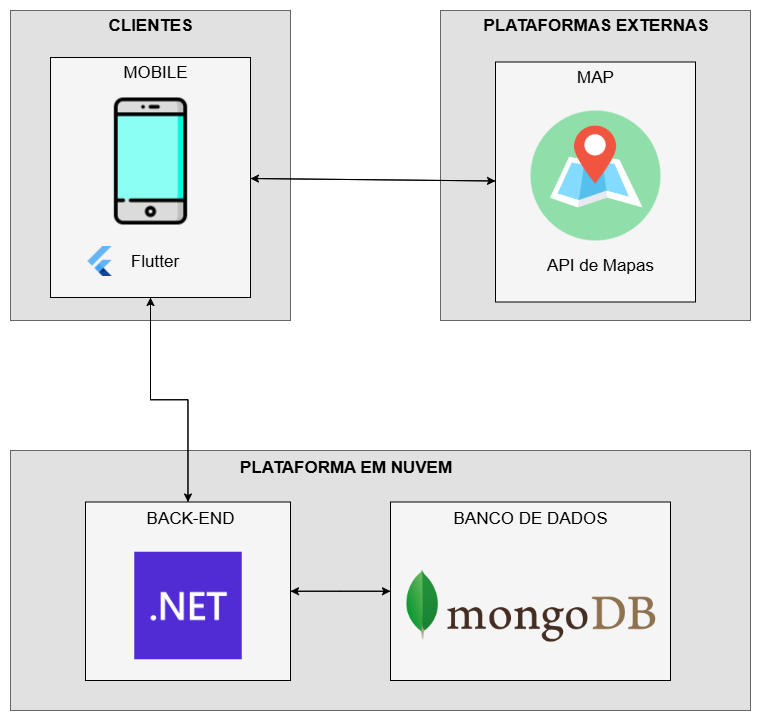
\includegraphics[scale=0.38]{./dados/figuras/diagrama-de-arquitetura.png}
    \fonte{\citeonline{DrawIO}}
\end{figure}

\section{PROTOTIPAGEM}
\label{sec:prototipagem}

Neste tópico vamos abordar a prototipagem, um processo extremamente necessário durante o desenvolvimento de um sistema. Segundo \citeonline{de2006prototipagem} a prototipagem tem a característica-chave de apresentar uma forma muito fácil de construir uma entidade temporária para que o produto possa ser visto é criticado, para então gerar novas melhorias.

É possível visualizar na \autoref{fig:prototipagemAutenticacaoUsuario} parte da prototipagem das telas relacionadas à autenticação de usuários, dentre elas estão: autenticação de usuário, registro de usuário e recuperação de senha.

\begin{figure}[H]
    \centering
    \caption{Prototipagem das Telas Relacionadas a Autenticação}
    \label{fig:prototipagemAutenticacaoUsuario}
    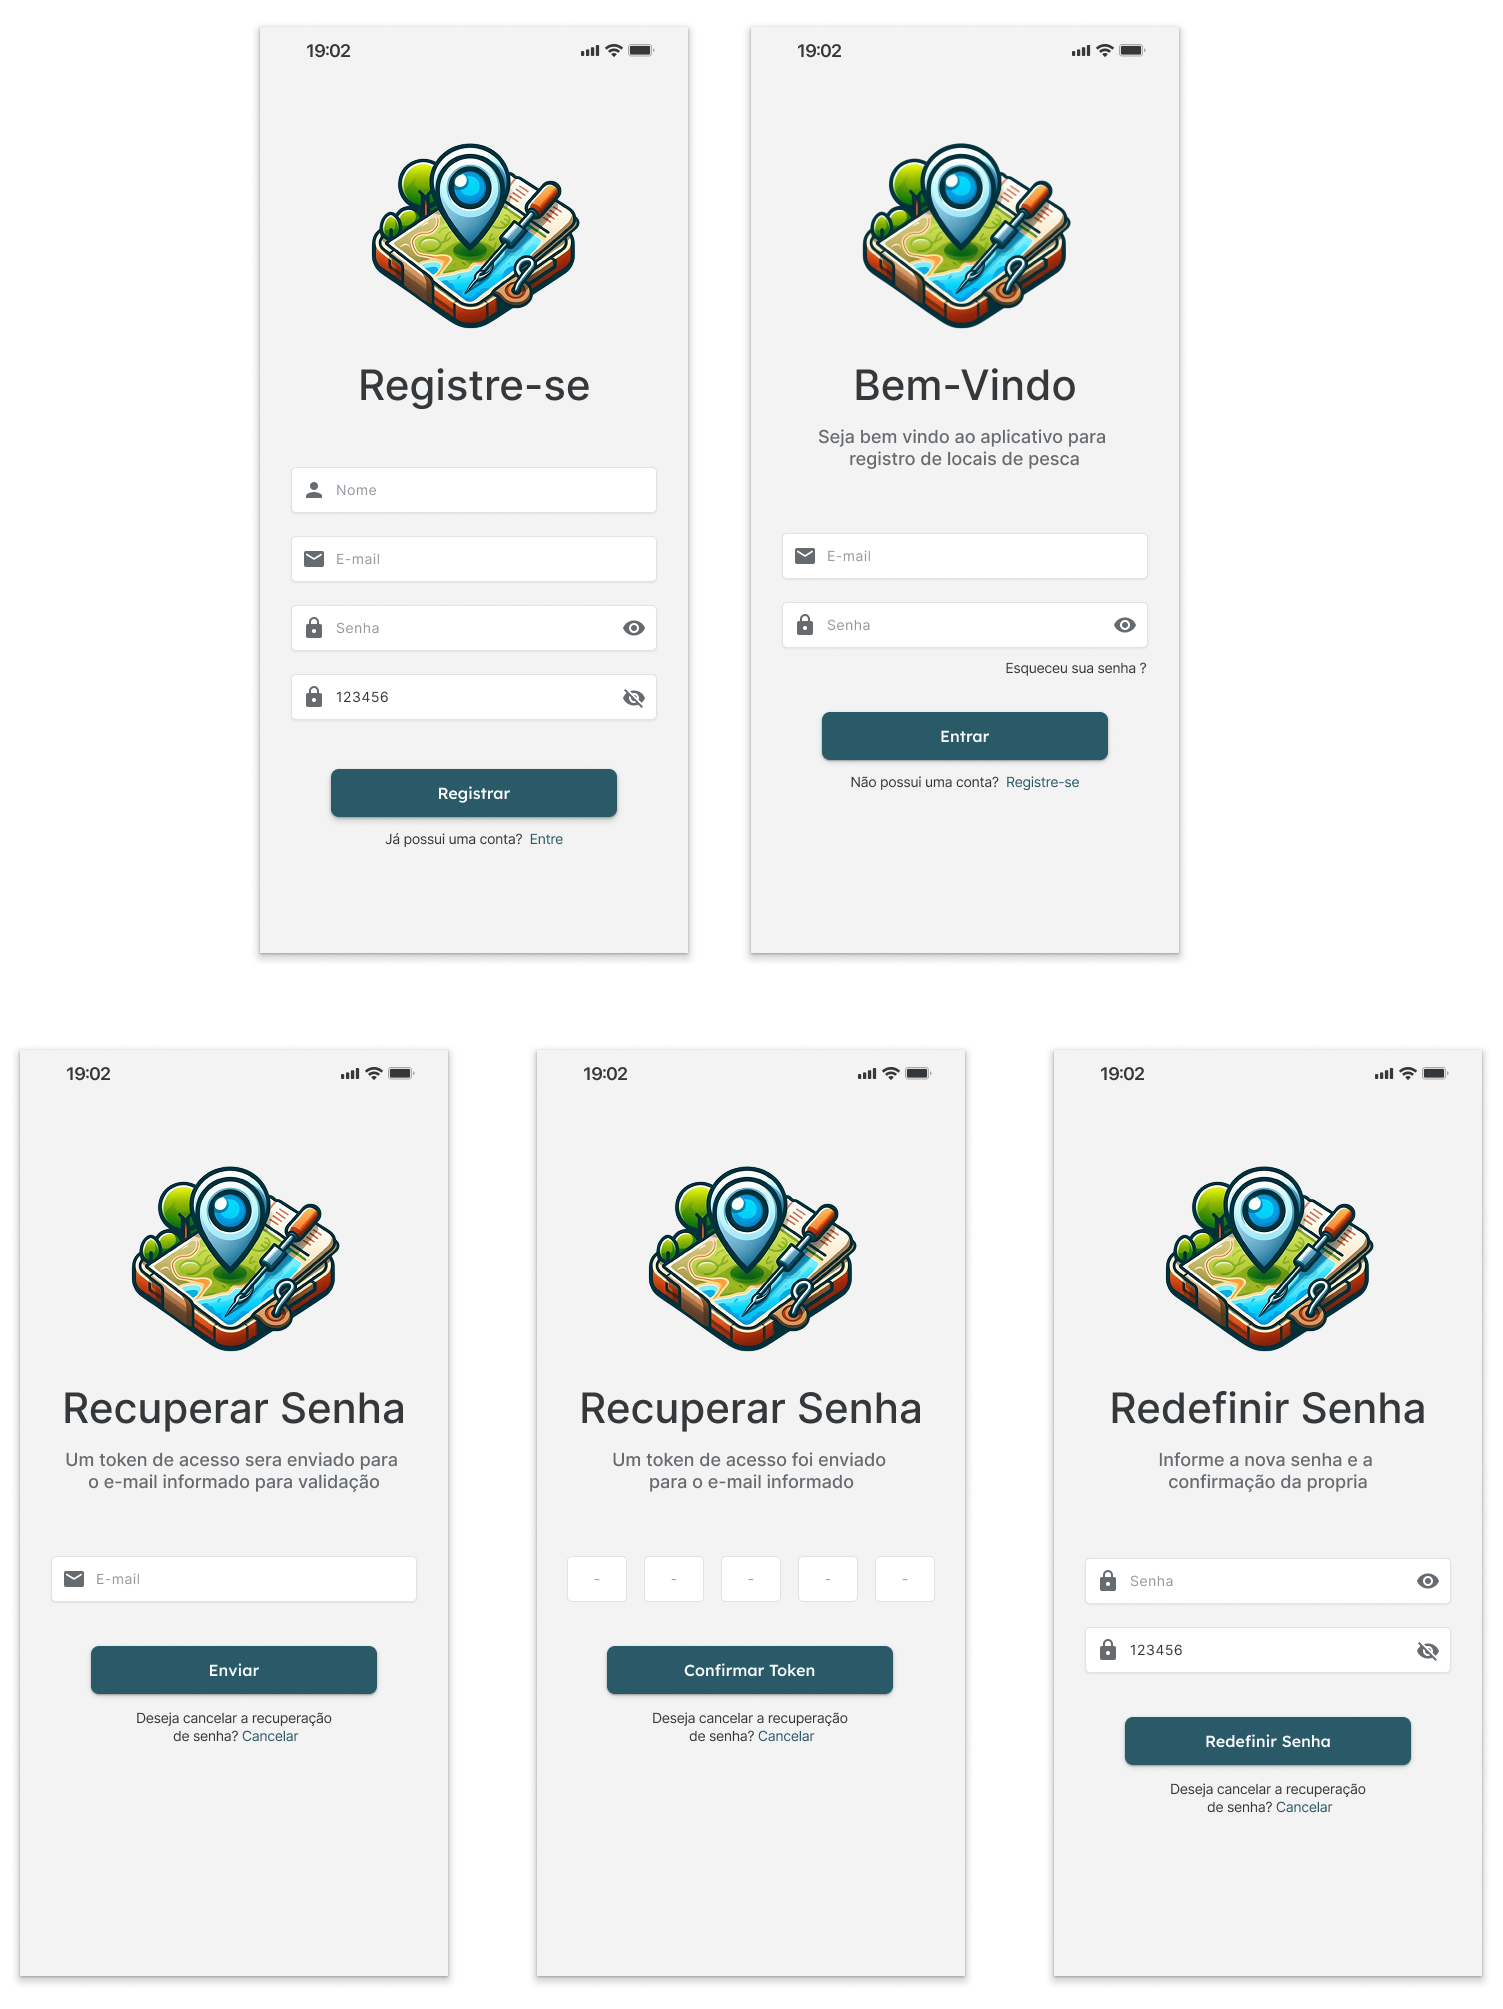
\includegraphics[scale=0.24]{./dados/figuras/prototipagem-autenticacao-de-usuario.png}
    \fonte{Produzido pelo Autor}
\end{figure}

A \autoref{fig:prototipagemMapPerfil} representa a prototipagem das telas relacionadas aos recursos de mapa e perfil do usuário, dentre elas estão o mapa, a visualização do ponto de pesca, perfil do pescador(a), edição do perfil do pescador(a) e uma futura tela de configuração.

\begin{figure}[H]
    \centering
    \caption{Prototipagem do Mapa e Perfil do Usuário}
    \label{fig:prototipagemMapPerfil}
    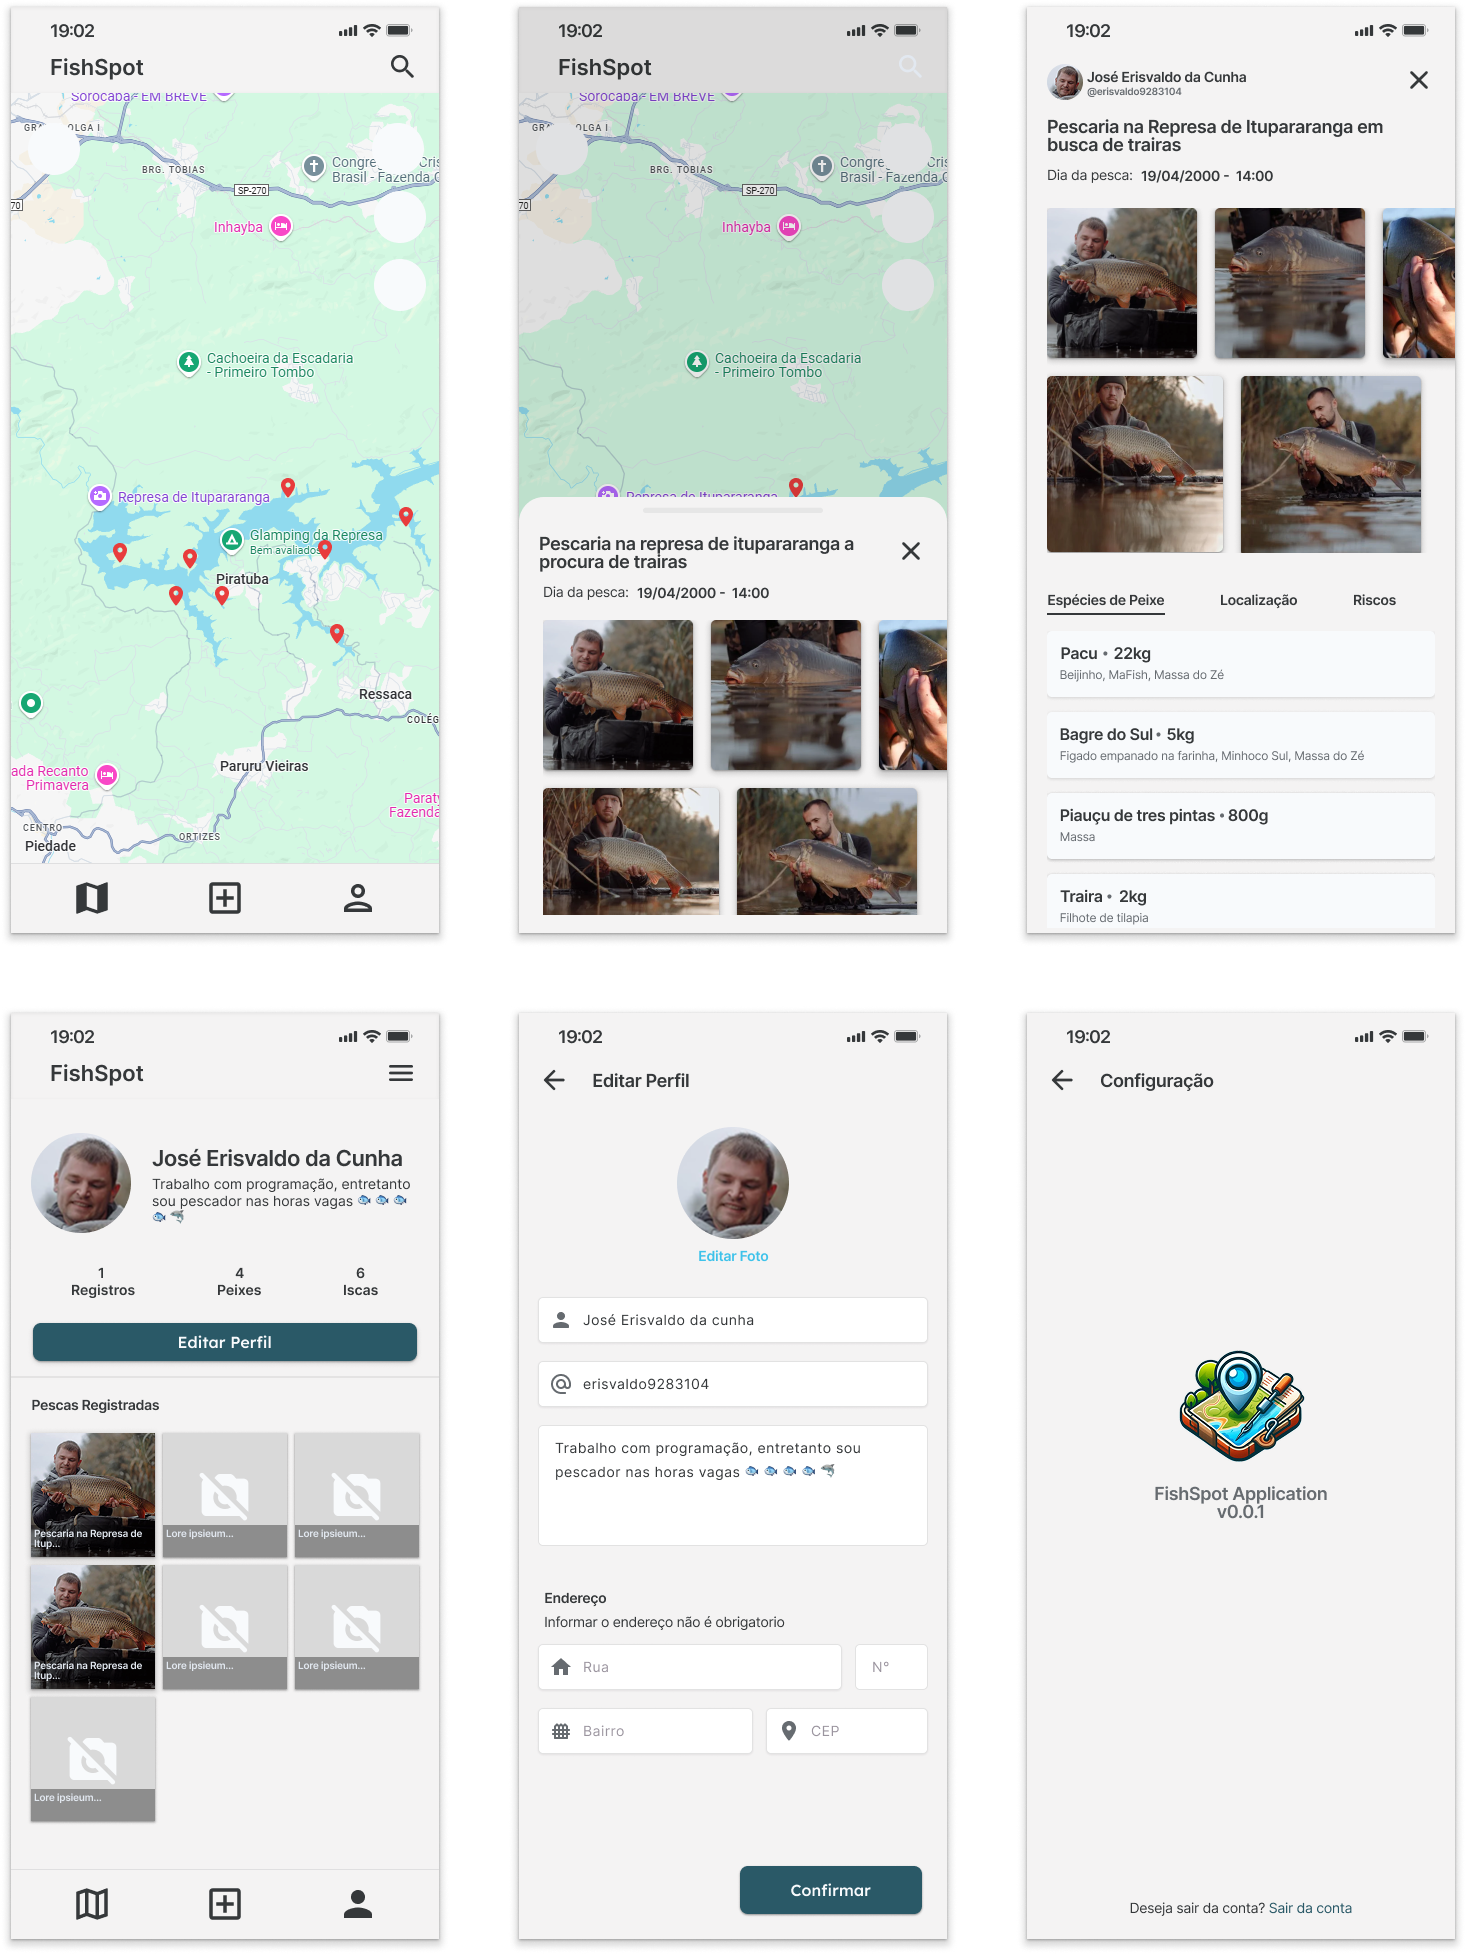
\includegraphics[scale=0.29]{./dados/figuras/prototipagem-map-perfil.png}
    \fonte{Produzido pelo Autor}
\end{figure}

A \autoref{fig:prototipagemRegisterSpot} apresenta a prototipagem das telas relacionadas ao registro dos pontos de pesca, dentre elas estão: descrição de riscos, inclusão de imagem, inclusão das iscas usadas e peixes pegos, inclusão de dados finais sobre o ponto.

\begin{figure}[H]
    \centering
    \caption{Prototipagem do Registro do Ponto de Pesca}
    \label{fig:prototipagemRegisterSpot}
    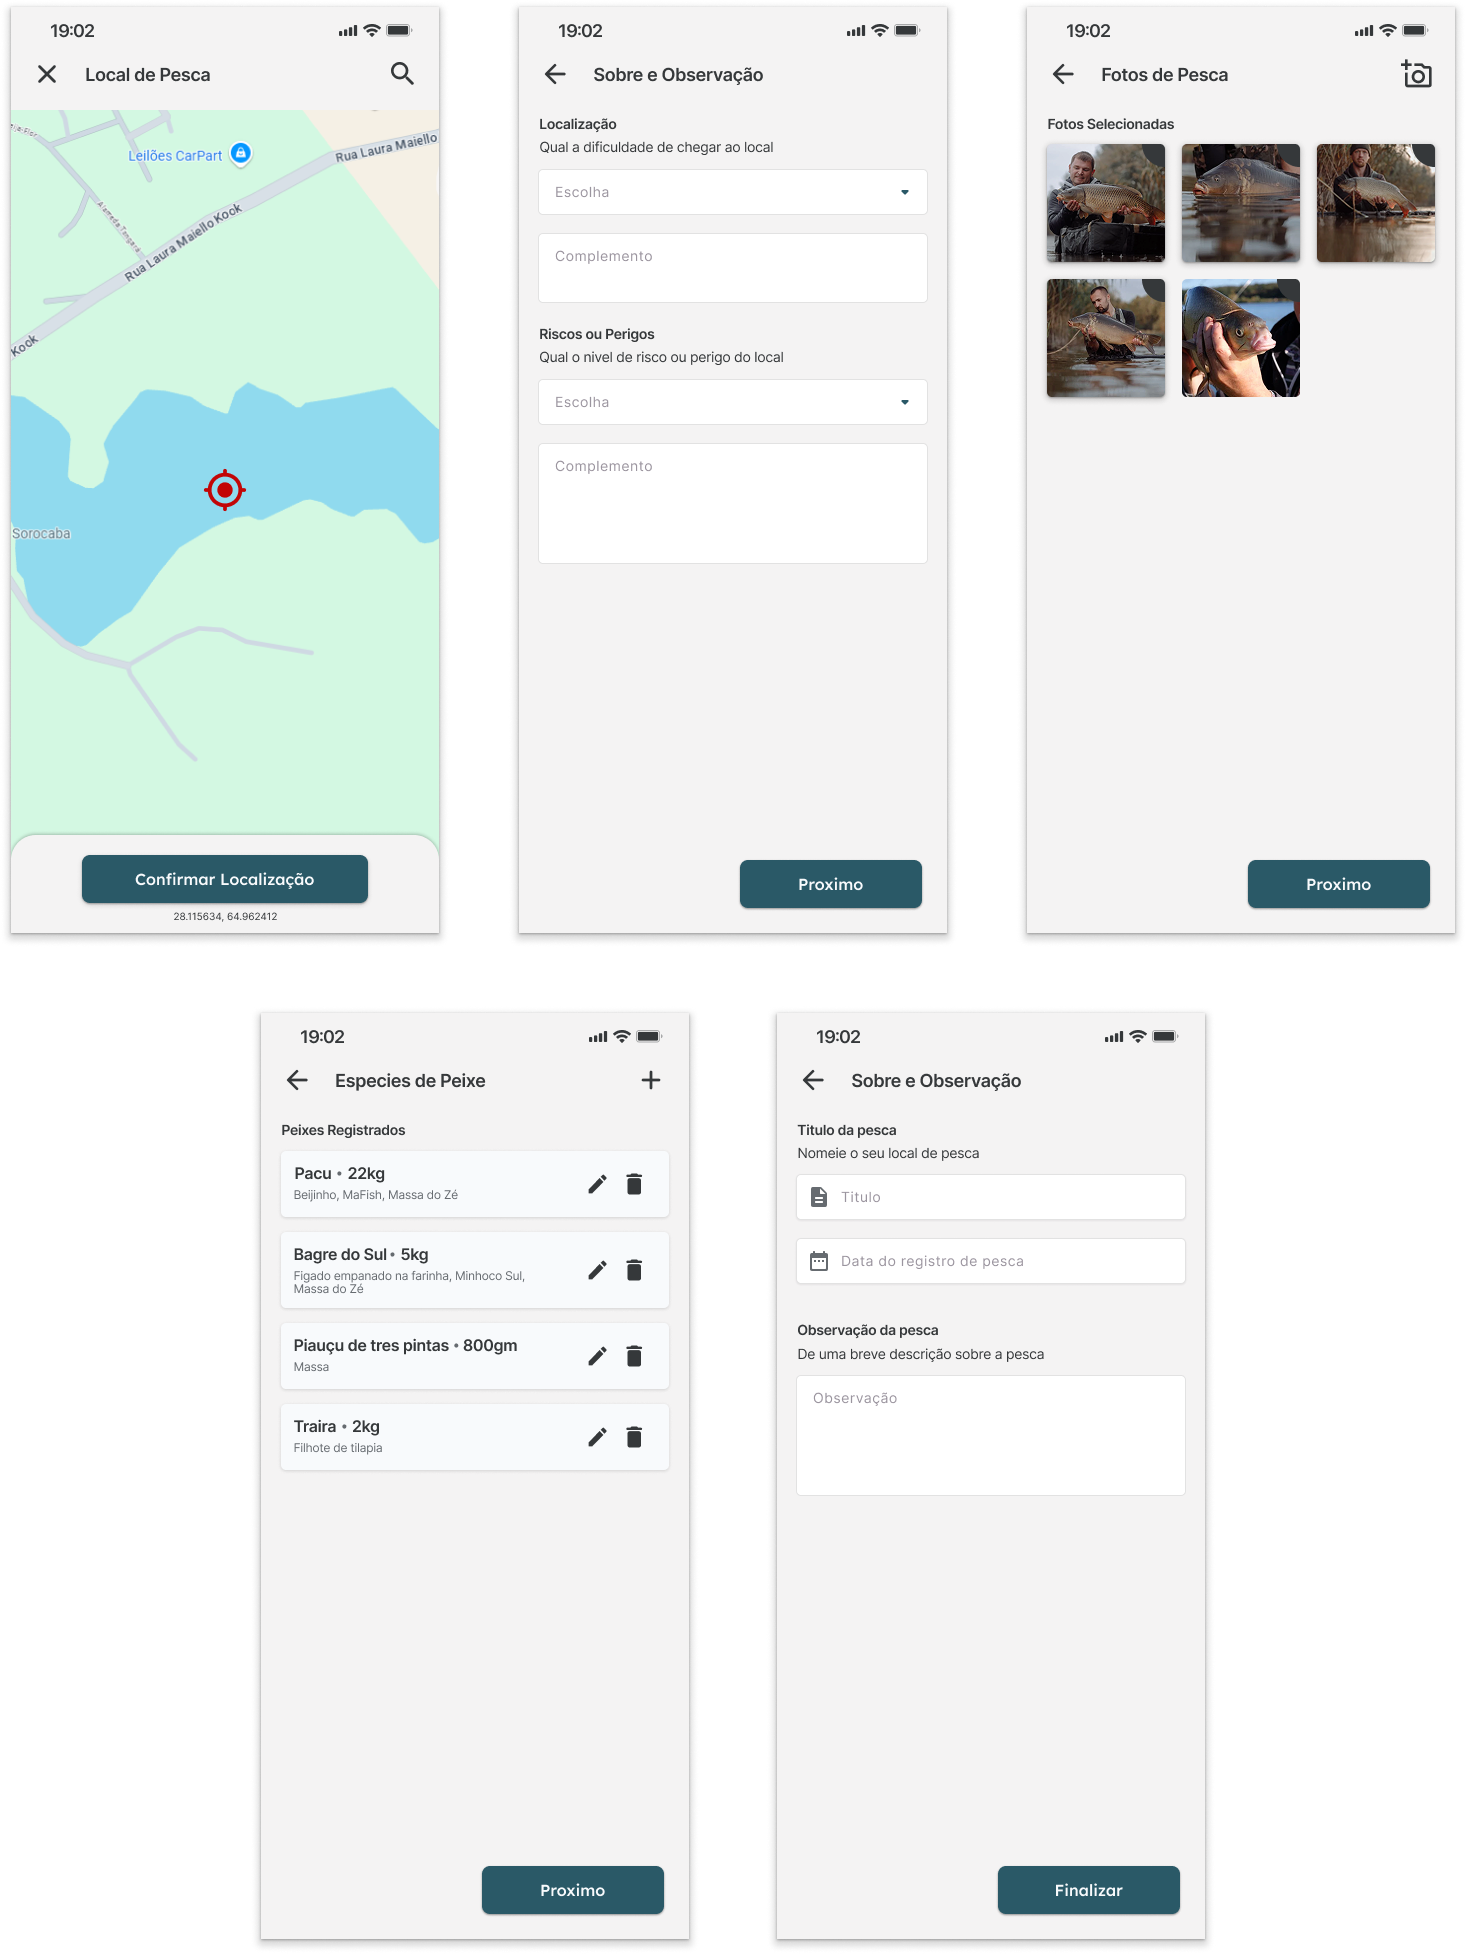
\includegraphics[scale=0.29]{./dados/figuras/prototipagem-spot-register.png}
    \fonte{Produzido pelo Autor}
\end{figure}


Pode-se observar na \autoref{fig:prototipagemAutenticacaoUsuarioDark} a prototipagem das telas de autenticação do usuário, destacando o modo escuro. Este que aumenta  usabilidade e cria maior conforto visual, reduzindo a fadiga ocular.

\begin{figure}[H]
    \centering
    \caption{Prototipagem das Telas Relacionadas a Autenticação no Modo Escuro}
    \label{fig:prototipagemAutenticacaoUsuarioDark}
    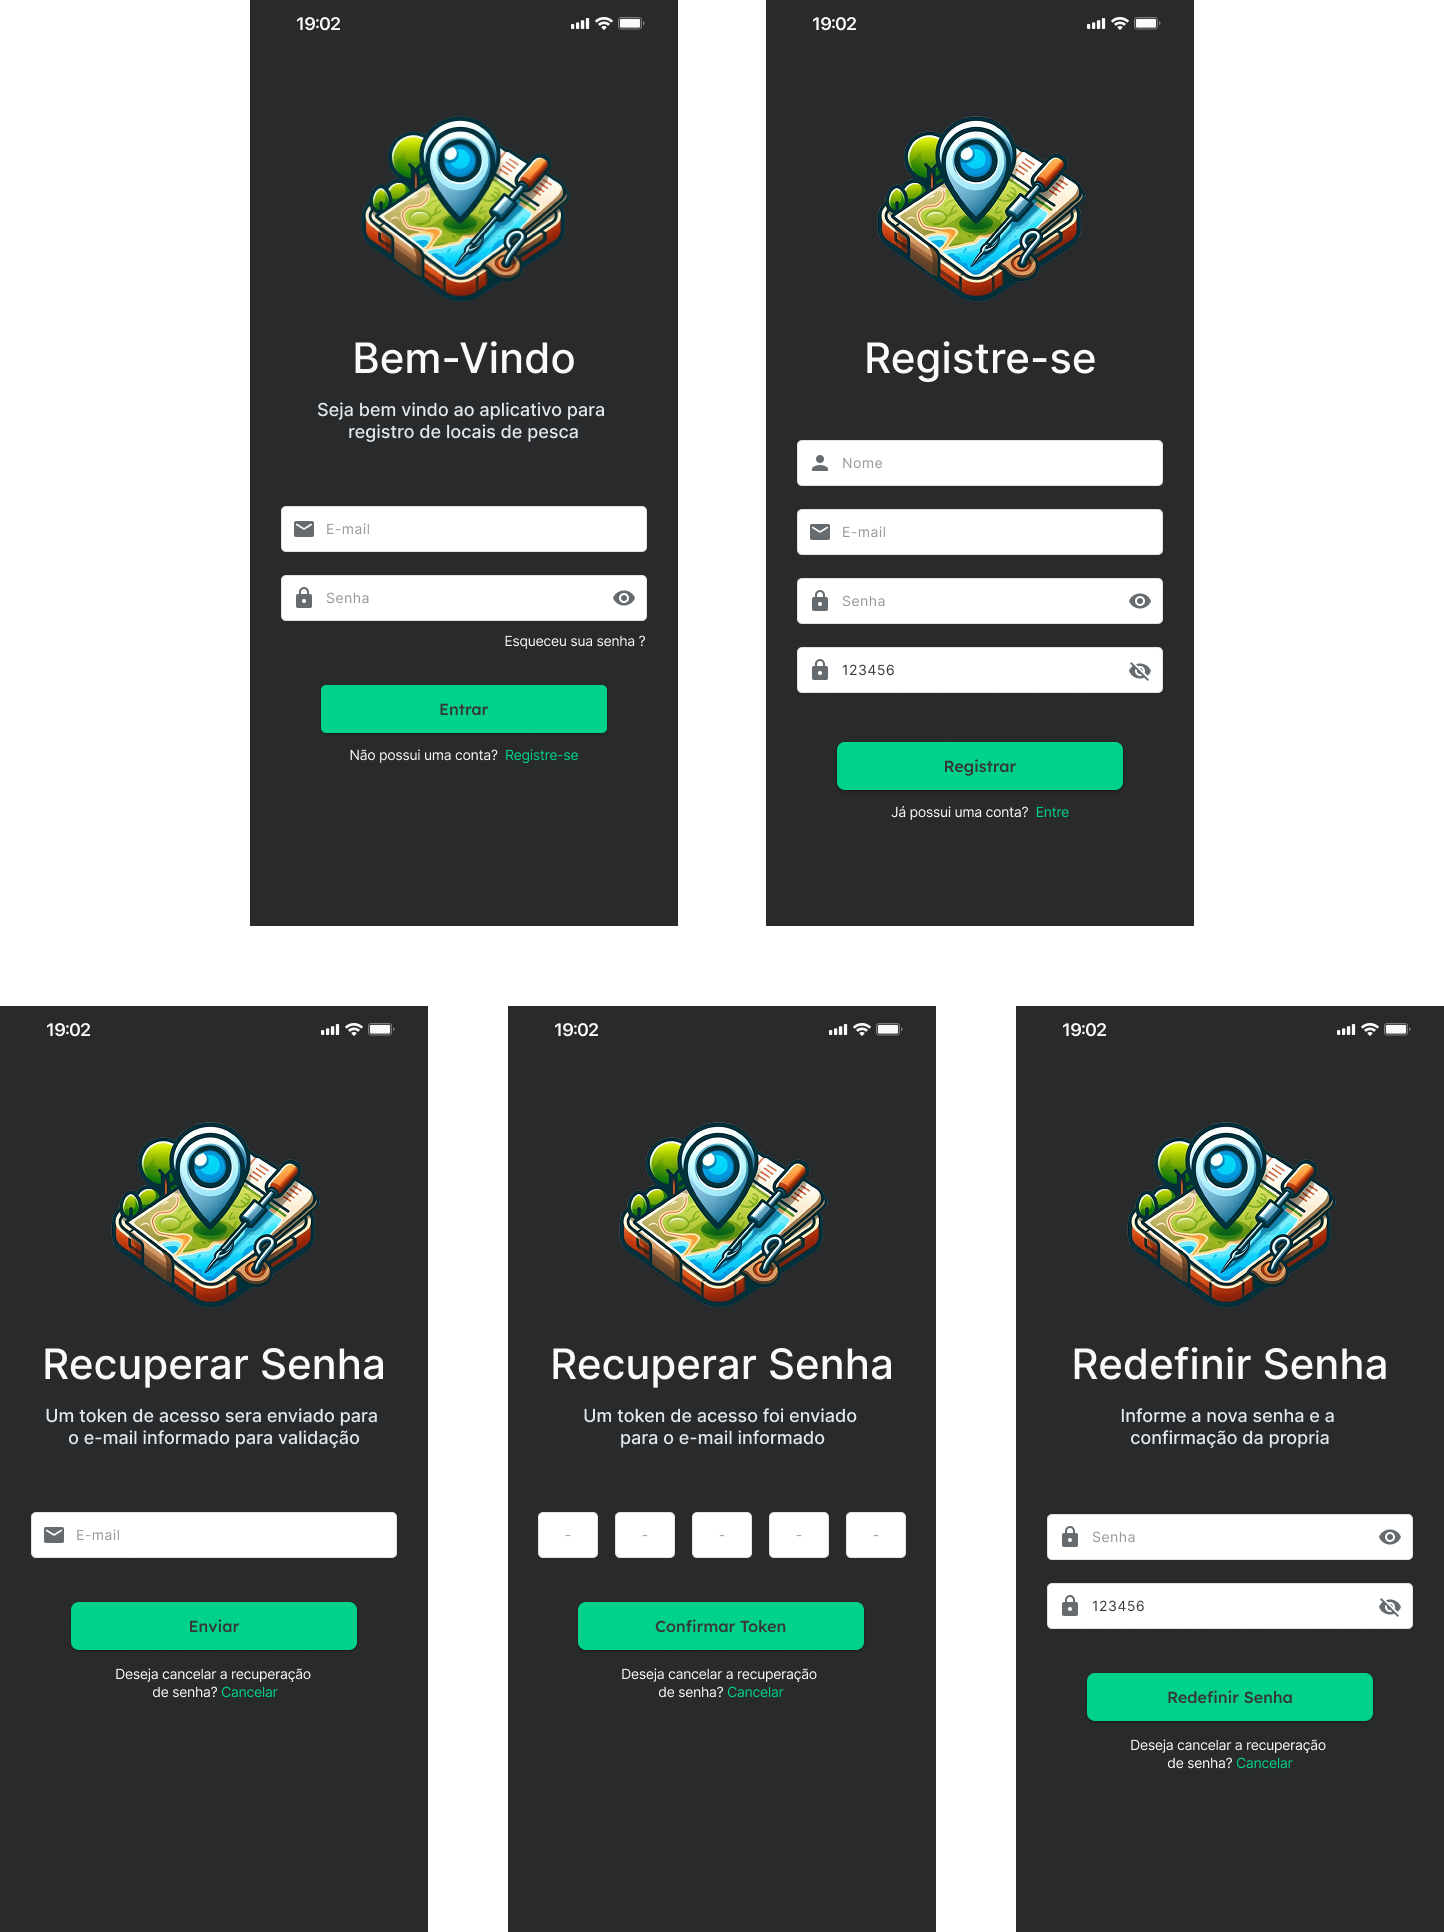
\includegraphics[scale=0.30]{./dados/figuras/prototipagem-dark-autenticacao-user.png}
    \fonte{Produzido pelo Autor}
\end{figure}

A \autoref{fig:prototipagemMapPerfilDark} exibe a prototipagem das telas de visualização dos pontos de pesca registrados, destacando o modo escuro da interface. Este que pode aumentar de forma significativa a economia no consumo de bateria do dispositivo móvel.

\begin{figure}[H]
    \centering
    \caption{Prototipagem do Mapa e Perfil do Usuário no Modo Escuro}
    \label{fig:prototipagemMapPerfilDark}
    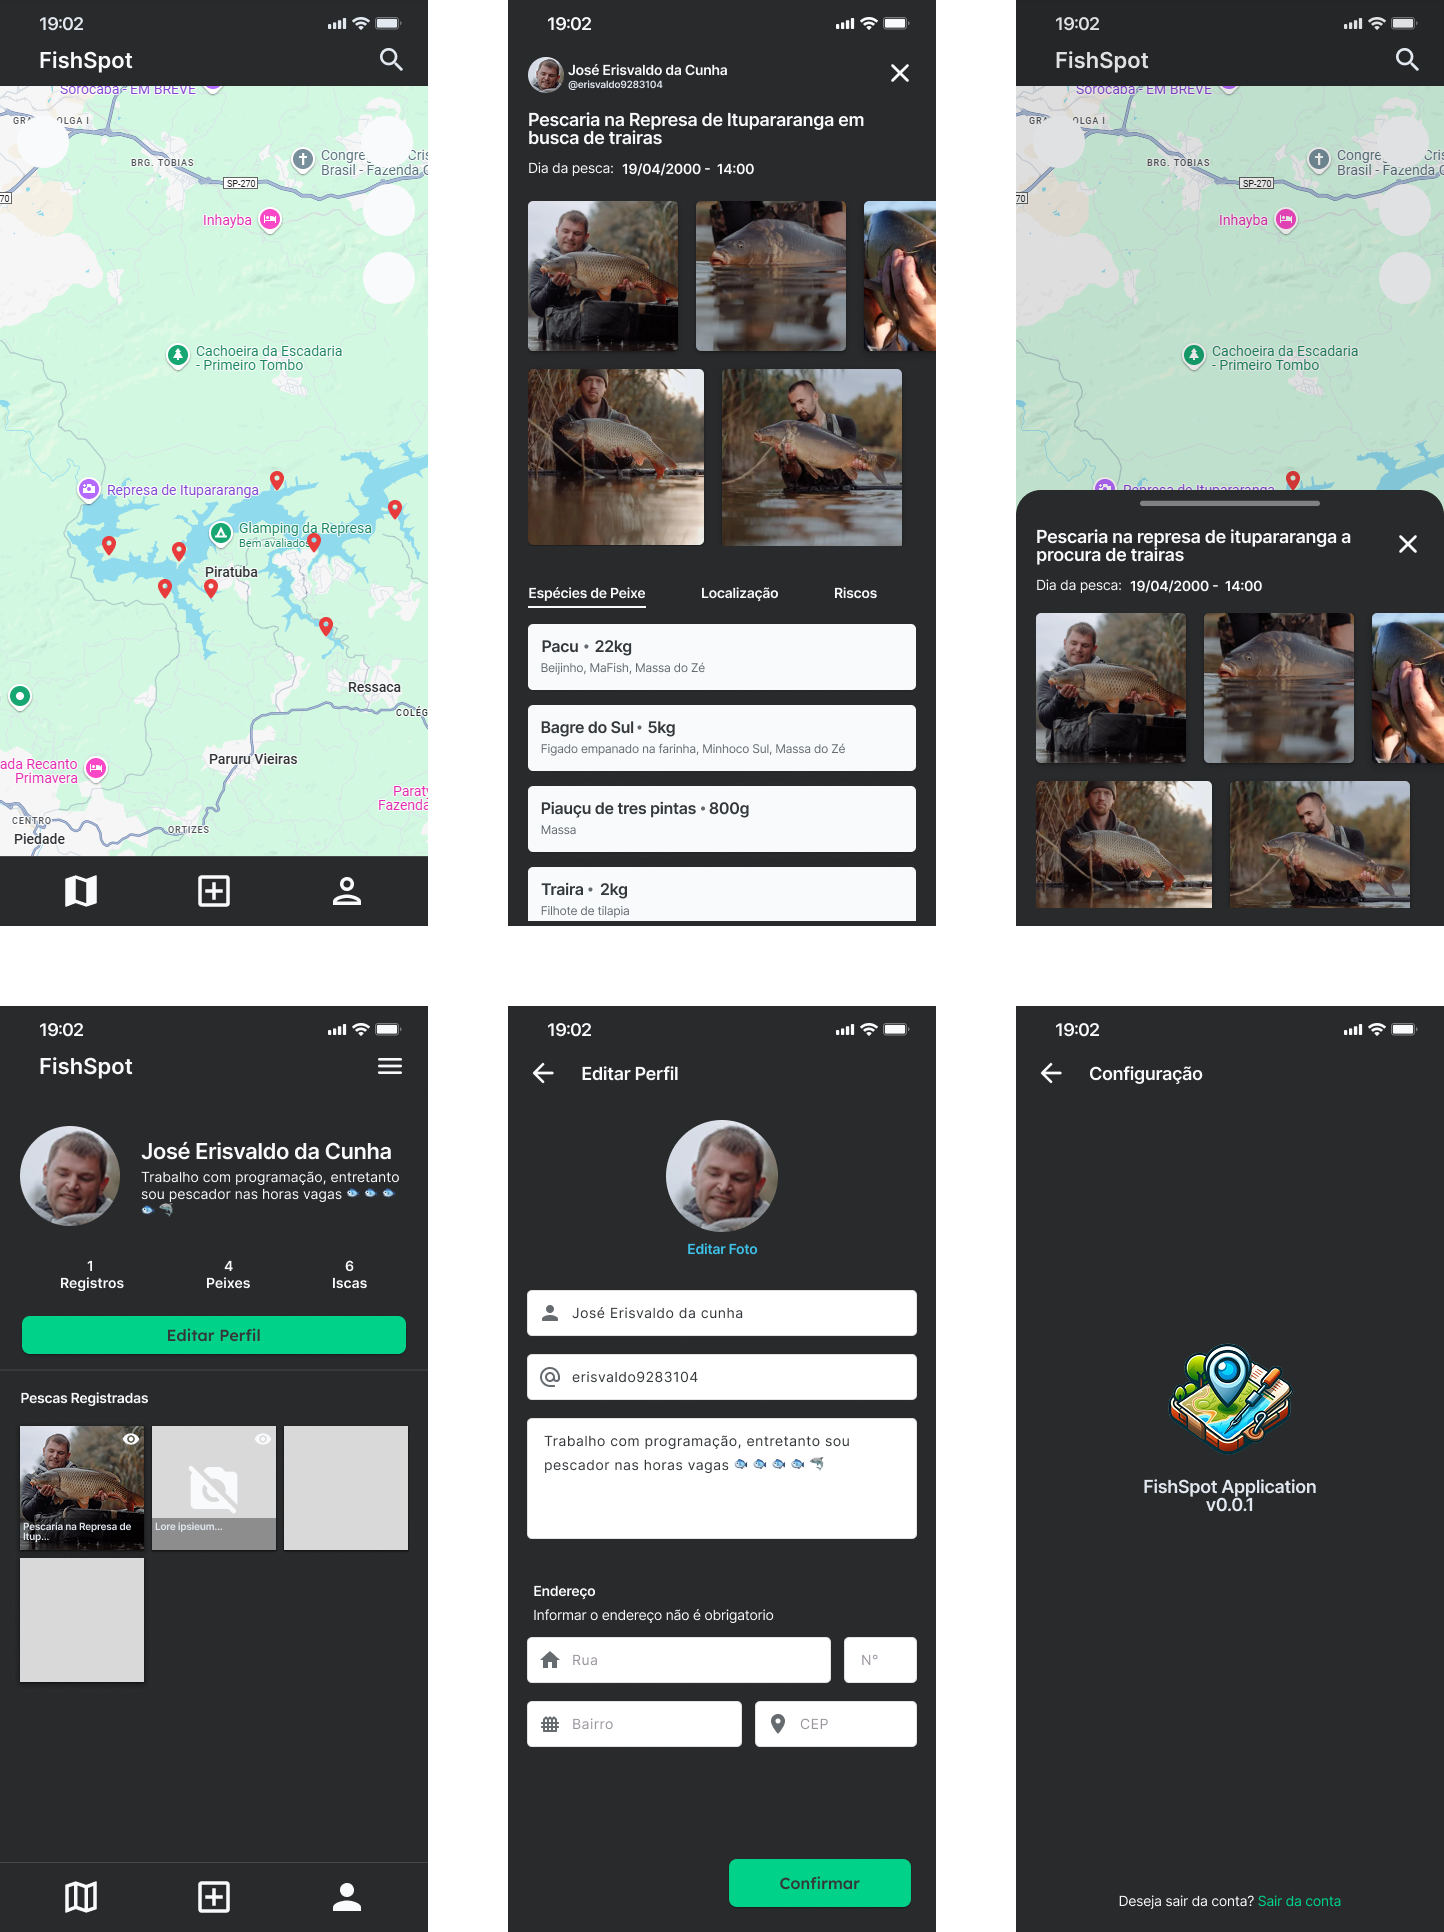
\includegraphics[scale=0.30]{./dados/figuras/prototipagem-dark-map-perfil.png}
    \fonte{Produzido pelo Autor}
\end{figure}

A \autoref{fig:prototipagemSpotRegisterDark} demonstra a prototipagem das telas de registro de pontos de pesca, destacando o modo escuro da interface. Este que busca atender às preferencias individuais e às necessidades de acessibilidade de diferentes usuários.

\begin{figure}[H]
    \centering
    \caption{Prototipagem do Registro do Ponto de Pesca no Modo Escuro}
    \label{fig:prototipagemSpotRegisterDark}
    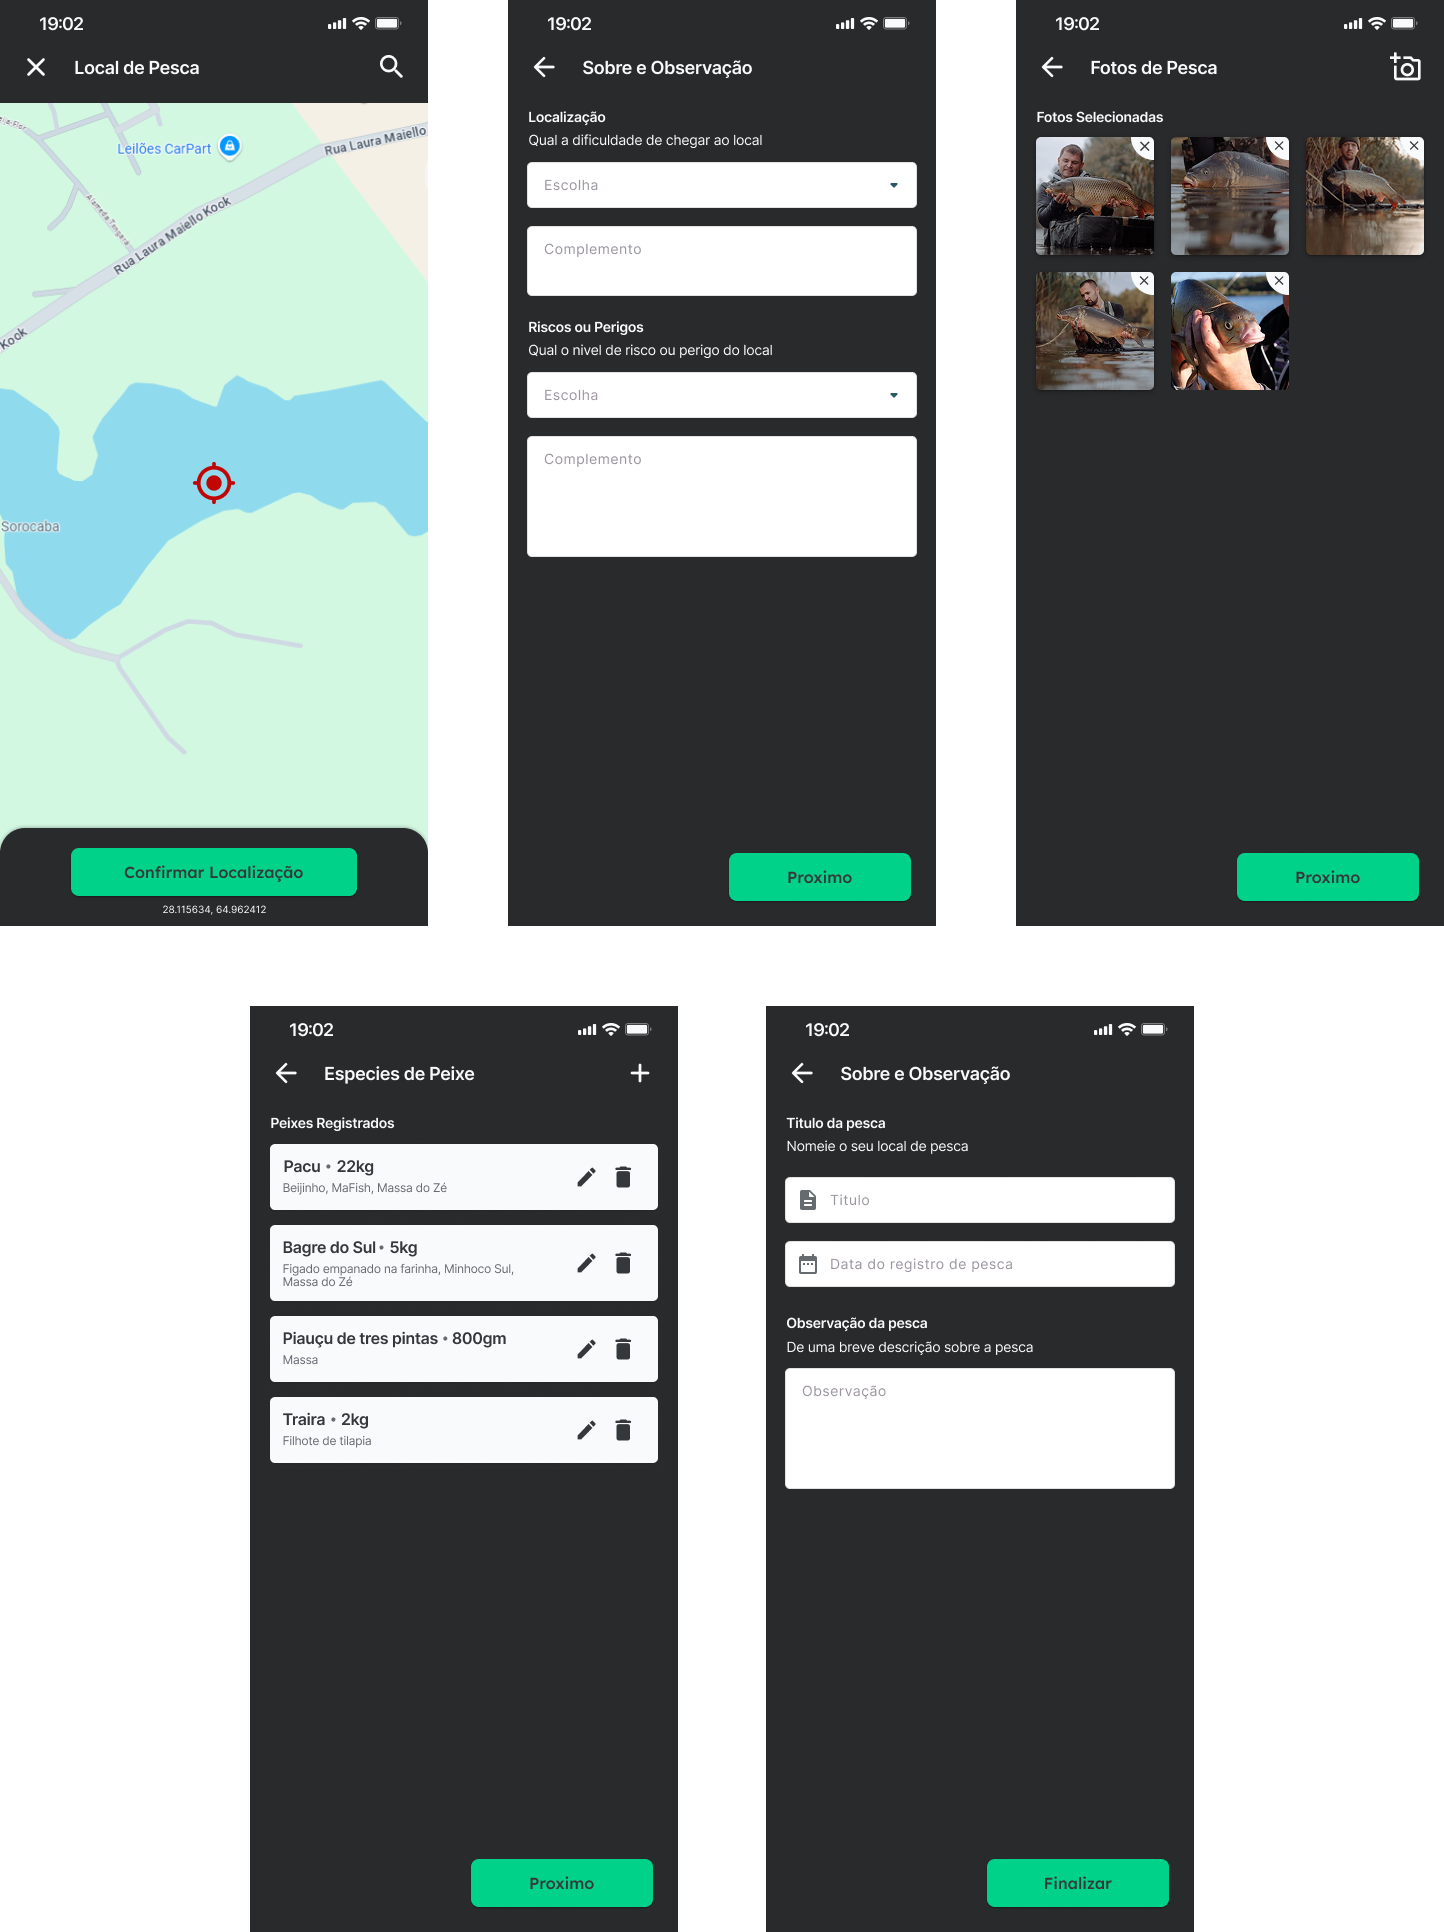
\includegraphics[scale=0.30]{./dados/figuras/prototipagem-dark-spot-register.png}
    \fonte{Produzido pelo Autor}
\end{figure}

\section{BANCO DE DADOS}
\label{sec:desenvolvimentobancodedados}

De acordo com a empresa \citeonline{MongoDBModelagem25}, detentora do banco de dados não relacional orientados a documento MongoDB. A criação de padroes de design de esquemas no banco de dados garantem de forma eficiente o armazenamento, a recuperação dos dados e a manipulação dos dados.

O diagrama ilustrado na \autoref{fig:documentacaoBancoDeDados}, representa a estrutura utilizado no banco de dados da aplicação, este que contem suas propriedades junto aos tipos utilizados, bem como sua relação.

\begin{figure}[H]
    \centering
    \caption{Documentação do Banco de Dados - MongoDB}
    \label{fig:documentacaoBancoDeDados}
    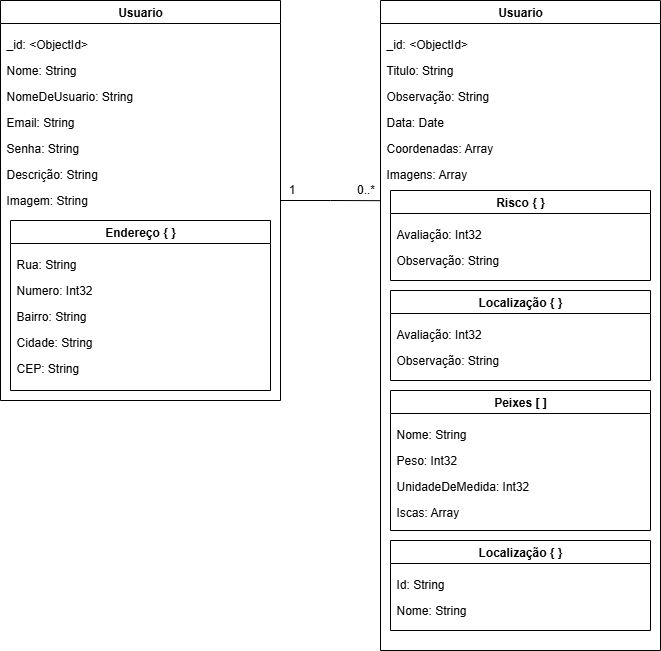
\includegraphics[scale=0.65]{./dados/figuras/documentacao-banco-de-dados.png}
    \fonte{Produzido pelo Autor}
\end{figure}